
\chapter{Teoria}
\label{cap:teoria}

\section{Els nombres naturals}

Els nombres acompanyen l'ésser humà des dels orígens del pensament. Tot va començar amb la necessitat de comptar. Si simbolitzem amb un palet $\vert$ la quantitat corresponent a una cosa, amb dos palets $\vert\vert$ representem dues coses, i així successivament. Cada símbol nou succeeix l'anterior afegint-hi un palet més, i és fàcil pensar que això és així indefinidament. Podríem considerar el conjunt format per la col·lecció d'aquests símbols i anomenar-lo el conjunt per a comptar objectes.

Ara bé, és evident que aquesta manera de fer-ho no és gens eficient; només cal pensar en una quantitat gran d'objectes. Tanmateix, podem millorar la nostra capacitat de recompte si agrupem els palets d'alguna manera. Per exemple, $\vert\vert\vert$ $\vert\vert\vert$ $\vert\vert\vert$ $\vert\vert\vert$ $\vert\vert$ simbolitza quatre agrupacions de tres palets més dos palets. Expressat aritmèticament, tenim $4\cdot 3+2=14$ palets. Si en lloc d'agrupar-los de 3 en 3 ho fem de 10 en 10, $\vert\vert\vert\vert\vert\vert\vert\vert\vert\vert$ $\vert\vert\vert\vert$, tenim $1\cdot 10+4=14$. I si la quantitat és molt gran podem agrupar-los també de 100 en 100, de 1000 en 1000, etc.

Aquesta idea és precisament la que dona lloc al sistema de numeració decimal, segons el qual fem ús dels dígits $0,1,2,3,4,5,6,7,8$ i $9$ per representar qualsevol quantitat. Quan escrivim $321$ volem expressar la quantitat
\[
1+2\cdot 10+3\cdot 100=321.
\]
Cal observar dos fets importants. En primer lloc, el sistema de numeració és \textbf{posicional}: les expressions $123$ i $132$ simbolitzen dues quantitats diferents ja que
\[
3+2\cdot 10+1\cdot 100\neq 2+3\cdot 10+1\cdot 100.
\]
En segon lloc, el dígit $0$ és imprescindible per poder distingir $107$ i $17$:
\[
1\cdot 100+0\cdot 10+7\neq 1\cdot 10+7.
\]
Observa en aquest últim cas que en $107$ hem fet una agrupació de $100$ i cap de $10$, mentre que en $17$ hem fet $1$ agrupació de $10$ i cap de $100$.

D'aquesta manera intuïtiva hem construït un conjunt de nombres que ens permet comptar quantitats o comptar objectes. Ara bé, des d'un punt de vista matemàtic aquesta forma d'introduir el conjunt no és prou rigorosa. Cal fer-ho mitjançant el llenguatge propi de les matemàtiques, tal com s'ha estudiat a \href{https://aprendes.com/batxillerat/logica/main.pdf}{\emph{Lògica, Raonament i Demostració}} i \href{https://aprendes.com/batxillerat/conjunts/main.pdf}{\emph{Conjunts, Relacions i Aplicacions}}. El que farem serà definir el conjunt dels nombres naturals per la seva \textbf{estructura} i no pel que són. Aquesta és precisament la idea que recullen els axiomes de Peano, que tractarem tot seguit.


\subsection{Axiomes de Peano}

Intuïtivament, els axiomes de Peano formalitzen la idea de comptar mitjançant cinc principis senzills:

\begin{enumerate}
\item Cal reconèixer que, a vegades, no cal comptar res.
\item Si hem comptat objectes i encara n'hi ha més, sempre podem comptar un objecte més.
\item No podem comptar un objecte més si no hi ha res.
\item Només hi ha una manera de comptar un objecte més.
\item Sempre comptem de la mateixa manera.
\end{enumerate}

Aquests cinc principis, expressats en forma matemàtica, donen lloc als axiomes que caracteritzen el conjunt dels nombres naturals.

Anomenem \textbf{conjunt dels nombres naturals}, i el denotem per $\N$, un conjunt dotat d’una aplicació $S:\N\rightarrow \N$, anomenada \textbf{successor}, que assigna a cada natural $n$ el seu \textbf{següent} o \textbf{successor} $S(n)$, i que compleix les propietats següents:

\begin{enumerate}
\item $0\in \N$.
\item Si $n\in \N$, aleshores $S(n)\in \N$.
\item No existeix $n\in \N$ tal que $S(n)=0$.
\item Si $S(m)=S(n)$, aleshores $m=n$.
\item Si $K\subseteq \N$, $0\in K$ i $\left( \forall n\right) \left(n\in K\implies S(n)\in K\right)$, llavors $K=\N$.
\end{enumerate}

El cinquè axioma es coneix com el \textbf{principi d'inducció} perquè permet establir propietats per a un nombre infinit de casos sense haver de donar un nombre infinit de proves. Concretament, si $P(n)$ és una propietat sobre $\N$ i comprovem que $P(0)$ és certa (\textbf{cas base}), i que per a cada $n\in \N$, si $P(n)$ és certa (\textbf{hipòtesi d'inducció}) llavors $P(S(n))$ també ho és (\textbf{pas inductiu}), aleshores el principi d'inducció ens permet concloure que $P(n)$ és certa per a tot $n\in \N$. Per això aquest principi és la base de les demostracions per inducció.

\begin{observacio}
Una manera equivalent d'introduir els nombres naturals és la següent. $\N$ és el conjunt amb les propietats:
\begin{enumerate}
\item $\N$ té un element distingit que simbolitzem per $0$. També es podria prendre $1$ com a element distingit, però aquí no ho farem perquè volem distingir clarament l'estructura algebraica de $\N$.
\item Hi ha una aplicació $S:\N\rightarrow \N$ anomenada successor.
\item $S$ és injectiva.
\item $0$ no pertany al recorregut de $S$. En particular, $S$ no és exhaustiva.
\item (Principi d'inducció) Si $K\subseteq \N$, $0\in K$ i $\left( \forall n\right) \left( n\in K\implies S(n)\in K\right)$, llavors $K=\N$.
\end{enumerate}
La propietat 3 és equivalent a l'axioma 4 original; la propietat 4 és equivalent a l'axioma 3; i la propietat 2 és equivalent a l’axioma 2.
\end{observacio}

Vegem ara un primer exemple senzill de com es treballa amb els axiomes de Peano.

\begin{exemple}
Provem que $4\neq 1$.
\end{exemple}

\begin{solucio}
Ho farem per reducció a l'absurd. Suposem que $4=1$. Aleshores
\[
S\left(S(S(S(0)))\right)=S(0).
\]
Aplicant l'axioma 4 de Peano, deduïm que $S(S(S(0)))=0$. Ara bé, això és impossible per l'axioma 3 de Peano, ja que $S(S(0))\in \N$ i el successor de cap natural no pot ser $0$. Per tant, queda provat que $4\neq 1$.
\end{solucio}

Vegem ara un altre exemple, aquest cop fent ús del principi d'inducció.

\begin{exemple}\label{3}
Si $n\in \N$ i $n\neq 0$, aleshores existeix $m\in \N$ tal que $S(m)=n$.
\end{exemple}

\begin{solucio}
Considerem la propietat
\[
P(n):=\text{``Si $n\in \N$ i $n\neq 0$, aleshores hi ha $m\in \N$ tal que $S(m)=n$''.}
\]
Volem provar que és certa per a tot $n\in \N$, i ho farem per inducció.

\textbf{Cas base.} $P(0)$ és certa perquè la implicació té antecedent fals (la hipòtesi $n\neq 0$ no es compleix quan $n=0$).

\textbf{Pas inductiu.} Suposem que $P(n)$ és certa (hipòtesi d'inducció). Volem veure que $P(S(n))$ també ho és. Ara bé, si $S(n)\neq 0$, podem prendre $m=n$ i tenim $S(m)=S(n)$ amb $m\in \N$, i per tant $P(S(n))$ és certa. Pel principi d'inducció, $P(n)$ és certa per a tot $n\in \N$.
\end{solucio}

\begin{exemple}
Si $n\in \N$, llavors o $n=0$ o bé $n$ s'obté aplicant $S$ a $0$ un nombre finit de vegades.
\end{exemple}

\begin{solucio}
Considerem la propietat
\[
P(n):=\text{``$n=0$ o $n$ s'obté aplicant $S$ a $0$ un nombre finit de vegades''.}
\]
Ho farem per inducció.

\textbf{Cas base.} $P(0)$ és certa de manera trivial.

\textbf{Pas inductiu.} Suposem $P(n)$ certa. Si $n=0$, llavors $S(n)=S(0)$, i $S(0)$ s'obté aplicant $S$ una vegada a $0$. Si $n\neq 0$, per hipòtesi d'inducció $n$ s'obté aplicant $S$ a $0$ un cert nombre $k$ de vegades. Aleshores $S(n)$ s'obté aplicant $S$ exactament una vegada més a $0$, és a dir, un nombre finit de vegades. Pel principi d'inducció, $P(n)$ és certa per a tot $n\in \N$.
\end{solucio}

El resultat de l'exemple anterior justifica que puguem escriure els nombres naturals com
\[
0,\ S(0),\ S(S(0)),\ S(S(S(0))),\ \ldots
\]
i, fent servir la notació tradicional,
\[
1:=S(0),\quad 2:=S(S(0)),\quad 3:=S(S(S(0))),\quad \ldots
\]
de manera que podem expressar el conjunt dels nombres naturals com
\[
\N=\{0,1,2,3,\ldots\}.
\]

\subsection{Recursió}

Els nombres naturals permeten introduir el concepte fonamental de \textbf{recursió}. Intuïtivament, diem que una definició és recursiva quan per determinar un objecte donem, d'una banda, un valor inicial i, de l'altra, una regla que permet obtenir el cas següent a partir del cas anterior.

Per exemple, podem definir una successió de nombres naturals $(u_n)_{n\in\N}$ de la manera següent:
\[
\left\{
\begin{array}{l}
u_0=0,\\
u_{S(n)}=S(u_n).
\end{array}
\right.
\]
Aquesta definició ens diu que el primer terme és $0$ i que cada terme següent s'obté prenent el successor del terme anterior. Així,
\[
u_0=0,\qquad
u_1=S(u_0)=S(0)=1,
\]
\[
u_2=S(u_1)=S(1)=2,\qquad
u_3=S(u_2)=S(2)=3,
\]
i així successivament.

Per tant, aquesta definició recursiva construeix la successió
\[
0,1,2,3,\ldots
\]
sense necessitat d'haver definit encara ni la suma ni la multiplicació.

Un altre exemple senzill de definició recursiva és el següent. Definim una successió de nombres naturals $(v_n)_{n\in\N}$ per
\[
\left\{
\begin{array}{l}
v_0=0,\\
v_{S(n)}=S(S(v_n)).
\end{array}
\right.
\]
Aquesta definició ens diu que el primer terme és $0$ i que cada terme següent s'obté aplicant dues vegades el successor al terme anterior. Així,
\[
v_0=0,
\]
\[
v_1=S(S(u_0))=S(S(0))=2,
\]
\[
v_2=S(S(v_1))=S(S(2))=4,
\]
\[
v_3=S(S(v_2))=S(S(4))=6,
\]
i així successivament.

D'aquesta manera obtenim la successió
\[
0,2,4,6,\ldots
\]

Observeu amb aquests exemples com hem definit successions de nombres naturals sense haver definit encara ni l'addició ni la multiplicació. Només hem fet servir el nombre inicial $0$ i l'aplicació successor.

\subsection{Addició de nombres naturals}

L'operació d'addició de nombres naturals es defineix per recursió. Tot i que la nostra intuïció ens permet entendre la definició sense dificultat, en un desenvolupament complet caldria justificar que existeix una única operació que compleix les regles següents. Aquesta justificació, però, l'ometrem aquí.

\begin{definicio}
Per a tots $a,b\in \N$ definim
\[
\left\{
\begin{array}{l}
a+0=a, \\
a+S(b)=S(a+b).
\end{array}
\right.
\]
El nombre natural $a+b$ s'anomena \textbf{suma} dels nombres $a$ i $b$, i diem que $a$ i $b$ són els \textbf{sumands}.
\end{definicio}

\subsubsection{Propietats de la suma}

Un conjunt dotat d'una operació és una \textbf{estructura algebraica}. Aquesta estructura s'anomena \textbf{monoide} quan l'operació és associativa i té element neutre. A més, si l'operació és commutativa, el monoide s'anomena \textbf{commutatiu}. Provarem tot seguit que els naturals tenen estructura de monoide commutatiu amb l'operació d'addició.

\begin{proposicio}
Per a tot $a\in \N$, $a+0=a$ i $0+a=a$. Això vol dir que $0$ és l'\textbf{element neutre} de la suma.
\end{proposicio}

\begin{prova}
La igualtat $a+0=a$ es compleix per definició. Per a la igualtat $0+a=a$, fem inducció sobre $a$.

\textbf{Cas base.} Si $a=0$, llavors $0+0=0$ per definició.

\textbf{Pas inductiu.} Suposem $0+a=a$ (hipòtesi d'inducció). Aplicant la definició i la hipòtesi d'inducció:
\[
0+S(a)=S(0+a)=S(a).
\]
Pel principi d'inducció, la propietat val per a tot $a\in \N$.
\end{prova}

\begin{observacio}\label{2}
A partir de la proposició anterior i de la definició podem escriure $S(n)=n+1$ per a tot $n\in \N$. En efecte,
\[
S(n)=S(n+0)=n+S(0)=n+1,
\]
perquè per notació $S(0):=1$.
\end{observacio}

Abans de demostrar les propietats associativa i commutativa de la suma, provarem la següent propietat.

\begin{proposicio}\label{prop:successor-suma}
Per a tots $a,b\in\N$, es compleix
\[
S(a)+b=S(a+b).
\]
\end{proposicio}

\begin{prova}
Fixem $a\in\N$ i demostrem la propietat per inducció sobre $b$.

Per a $b=0$, tenim
\[
S(a)+0=S(a),
\]
per la definició de la suma. D'altra banda,
\[
S(a+0)=S(a),
\]
ja que $a+0=a$. Per tant,
\[
S(a)+0=S(a+0).
\]

Suposem ara que la propietat és certa per a un cert $b\in\N$, és a dir,
\[
S(a)+b=S(a+b).
\]
Volem demostrar que també és certa per a $S(b)$.

Per la definició de la suma,
\[
S(a)+S(b)=S(S(a)+b).
\]
Per la hipòtesi d'inducció,
\[
S(S(a)+b)=S(S(a+b)).
\]
D'altra banda, com que
\[
a+S(b)=S(a+b),
\]
tenim
\[
S(a+S(b))=S(S(a+b)).
\]
Així,
\[
S(a)+S(b)=S(a+S(b)).
\]

Per tant, la propietat és certa per a $S(b)$. Pel principi d'inducció, queda provat que
\[
S(a)+b=S(a+b)
\]
per a tots $a,b\in\N$.
\end{prova}

\begin{proposicio}
Per a tots $a,b,c\in \N$, la suma és \textbf{associativa}:
\[
a+(b+c)=(a+b)+c,
\]
i \textbf{commutativa}:
\[
a+b=b+a.
\]
\end{proposicio}

\begin{prova}
\textbf{Associativitat.} Fem inducció sobre $c$.

\textbf{Cas base.} Si $c=0$, llavors $a+(b+0)=a+b=(a+b)+0$ per definició.

\textbf{Pas inductiu.} Suposem $a+(b+c)=(a+b)+c$. Aleshores
\[
a+(b+S(c))=a+S(b+c)=S(a+(b+c))=S((a+b)+c)=(a+b)+S(c).
\]

\textbf{Commutativitat.} Fem inducció sobre $b$.

\textbf{Cas base.} Si $b=0$, per la proposició anterior $a+0=0+a=a$.

\textbf{Pas inductiu.} Suposem $a+b=b+a$. Aleshores,

\begin{align*}
a+S(b) 
&= S(a+b)
&& \text{per definició de suma} \\
&= S(b+a)
&& \text{per la hipòtesi d'inducció} \\
&= S(b) + a 
&& \text{per la proposició~\ref{prop:successor-suma}}.
\end{align*}
\end{prova}

\begin{exemple}[Propietat de simplificació]
Per a tots $a,b,c\in \N$, si $c+a=c+b$, aleshores $a=b$.
\end{exemple}

\begin{solucio}
Fem inducció sobre $c$.

\textbf{Cas base.} Si $c=0$, llavors $0+a=0+b$, així que $a=b$.

\textbf{Pas inductiu.} Suposem que $c+a=c+b$ implica $a=b$. Volem provar que $S(c)+a=S(c)+b$ també implica $a=b$. En efecte, per la commutativitat de la suma:
\[
S(c)+a=S(c)+b \implies a+S(c)=b+S(c) \implies S(a+c)=S(b+c).
\]
Per l'axioma 4 de Peano, $a+c=b+c$, i de nou per commutativitat $c+a=c+b$. Per la hipòtesi d'inducció, $a=b$.
\end{solucio}

\subsection{Multiplicació de nombres naturals}

La multiplicació de nombres naturals també es defineix per recursió. Igual que abans, no justificarem aquí l'existència i la unicitat d’aquesta operació.

\begin{definicio}
Per a tots $a,b\in \N$ definim
\[
\left\{
\begin{array}{l}
a\cdot 0=0, \\
a\cdot S(b)=a\cdot b+a.
\end{array}
\right.
\]
El nombre natural $a\cdot b$ s'anomena \textbf{producte} dels nombres $a$ i $b$, i $a$ i $b$ s'anomenen \textbf{factors}.
\end{definicio}

\subsubsection{Propietats de la multiplicació}

Igual que el conjunt dels naturals té estructura de monoide commutatiu amb la suma, també té estructura de monoide commutatiu amb la multiplicació. A més, la multiplicació és distributiva respecte de la suma.

\begin{proposicio}
Per a tot $a\in \N$, $a\cdot 0=0$ i $0\cdot a=0$.
\end{proposicio}

\begin{prova}
La igualtat $a\cdot 0=0$ es compleix per definició. Per a la igualtat $0\cdot a=0$, fem inducció sobre $a$.

\textbf{Cas base.} Si $a=0$, és immediat que $0\cdot 0=0$ per definició.

\textbf{Pas inductiu.} Suposem $0\cdot a=0$. Aplicant la definició de multiplicació i la propietat de l'element neutre de la suma:
\[
0\cdot S(a)=0\cdot a+0=0+0=0.
\]
Per tant, $0\cdot a=0$ per a tot $a\in \N$.
\end{prova}

\begin{proposicio}
Per a tot $a\in \N$, $a\cdot 1=a$ i $1\cdot a=a$. Això vol dir que $1$ és l'\textbf{element neutre} de la multiplicació.
\end{proposicio}

\begin{prova}
En primer lloc, aplicant que $S(0)=1$, la definició de multiplicació i la propietat de l'element neutre de la suma:
\[
a\cdot 1=a\cdot S(0)=a\cdot 0+a=0+a=a.
\]
Per a la igualtat $1\cdot a=a$, fem inducció sobre $a$.

\textbf{Cas base.} Si $a=0$, $1\cdot 0=0$ per la proposició anterior.

\textbf{Pas inductiu.} Suposem $1\cdot a=a$. Aleshores
\[
1\cdot S(a)=1\cdot a+1=a+1=a+S(0)=S(a+0)=S(a).
\]
\end{prova}

\begin{proposicio}
Per a tot $a,b,c\in \N$, la multiplicació és \textbf{associativa},
\[
a\cdot (b\cdot c)=(a\cdot b)\cdot c,
\]
i \textbf{distributiva respecte de la suma},
\[
a\cdot (b+c)=a\cdot b+a\cdot c.
\]
\end{proposicio}

\begin{prova}
\textbf{Distributivitat.} Fem inducció sobre $c$.

\textbf{Cas base.} Si $c=0$, és immediat que $a\cdot (b+0)=a\cdot b=a\cdot b+a\cdot 0$.

\textbf{Pas inductiu.} Suposem $a\cdot (b+c)=a\cdot b+a\cdot c$. Aleshores
\[
\begin{array}{lll}
a\cdot (b+S(c)) &=& a\cdot S(b+c)\\
&=& a\cdot (b+c)+a\\
&=& (a\cdot b+a\cdot c)+a\\
&=& a\cdot b+(a\cdot c+a)\\
&=& a\cdot b+a\cdot S(c).
\end{array}
\]

\textbf{Associativitat.} Fem inducció sobre $c$.

\textbf{Cas base.} Si $c=0$, $a\cdot (b\cdot 0)=(a\cdot b)\cdot 0=0$.

\textbf{Pas inductiu.} Suposem $a\cdot (b\cdot c)=(a\cdot b)\cdot c$. Aplicant la definició de multiplicació i la propietat distributiva:
\[
\begin{array}{lll}
a\cdot (b\cdot S(c)) &=& a\cdot (b\cdot c+b)\\
&=& a\cdot (b\cdot c)+a\cdot b\\
&=& (a\cdot b)\cdot c+a\cdot b\\
&=& (a\cdot b)\cdot S(c).
\end{array}
\]
\end{prova}

Abans de demostrar la propietat commutativa de la multiplicació, provarem la propietat següent.

\begin{proposicio}\label{prop:successor-producte-primer-factor}
Per a tots $a,b\in\N$, es compleix
\[
S(a)\cdot b=a\cdot b+b.
\]
\end{proposicio}

\begin{prova}
Fixem $a\in\N$ i demostrem la propietat per inducció sobre $b$.

Per a $b=0$, tenim
\[
S(a)\cdot 0=0,
\]
per la definició del producte. D'altra banda,
\[
a\cdot 0+0=0+0=0.
\]
Per tant,
\[
S(a)\cdot 0=a\cdot 0+0.
\]

Suposem ara que la propietat és certa per a un cert $b\in\N$, és a dir,
\[
S(a)\cdot b=a\cdot b+b.
\]
Volem demostrar que també és certa per a $S(b)$.

Per la definició del producte,
\[
S(a)\cdot S(b)=S(a)\cdot b+S(a).
\]
Per la hipòtesi d'inducció,
\[
S(a)\cdot S(b)=(a\cdot b+b)+S(a).
\]
Per l'associativitat de la suma,
\[
(a\cdot b+b)+S(a)=a\cdot b+(b+S(a)).
\]
Ara bé, per la definició de la suma i per la commutativitat de la suma,
\[
b+S(a)=S(b+a)=S(a+b)=a+S(b).
\]
Així,
\[
S(a)\cdot S(b)=a\cdot b+(a+S(b)).
\]
Per l'associativitat de la suma,
\[
a\cdot b+(a+S(b))=(a\cdot b+a)+S(b).
\]
Finalment, per la definició del producte,
\[
a\cdot b+a=a\cdot S(b).
\]
Per tant,
\[
S(a)\cdot S(b)=a\cdot S(b)+S(b).
\]

Això prova la propietat per a $S(b)$. Pel principi d'inducció, queda demostrat que
\[
S(a)\cdot b=a\cdot b+b
\]
per a tots $a,b\in\N$.
\end{prova}

\begin{proposicio}
La multiplicació és \textbf{commutativa}: $a\cdot b=b\cdot a$ per a tots $a,b\in \N$.
\end{proposicio}

\begin{prova}
Fem inducció sobre $b$.

\textbf{Cas base.} Si $b=0$, és clar que $a\cdot 0=0\cdot a=0$.

\textbf{Pas inductiu.} Suposem $a\cdot b=b\cdot a$. Aleshores,

\begin{align*}
a\cdot S(b) 
&= a\cdot b+a 
&& \text{per definició del producte} \\
&= b\cdot a+a 
&& \text{per la hipòtesi d'inducció} \\
&= S(b)\cdot a 
&& \text{per la proposició~\ref{prop:successor-producte-primer-factor}}.
\end{align*}
\end{prova}

\begin{exemple}
Per a tot $a\in \N$ es compleix $S(a)\neq a$.
\end{exemple}

\begin{solucio}
Fem inducció sobre $a$.

\textbf{Cas base.} Si $a=0$, $S(0)\neq 0$ per l'axioma 3 de Peano.

\textbf{Pas inductiu.} Suposem $S(a)\neq a$. Pel contrarecíproc de l'axioma 4 de Peano, si $S(a)\neq a$, llavors $S(S(a))\neq S(a)$. Per tant, la propietat també és certa per a S(a).
\end{solucio}

\begin{exemple}[El factorial]
Definim el factorial d'un nombre natural per recursió:
\[
\left\{
\begin{array}{l}
0!:=1, \\
S(n)!:=S(n)\cdot n!.
\end{array}
\right.
\]
Així,
\[
0!=1,
\]
\[
1!=S(0)!=S(0)\cdot 0!=1\cdot 1=1,
\]
\[
2!=S(1)!=S(1)\cdot 1!=2\cdot 1=2,
\]
\[
3!=S(2)!=S(2)\cdot 2!=3\cdot 2=6.
\]
\end{exemple}

\begin{exemple}
Expressa per recursió la successió de Fibonacci
\[
f=(0,1,1,2,3,5,8,13,\ldots).
\]
Per fer-ho, observa que cada terme a partir del tercer s'obté com a suma dels dos termes anteriors.
\end{exemple}

\begin{solucio}
Per a tot $n\in \N$ definim:
\[
\left\{
\begin{array}{l}
f(0)=0, \\
f(1)=1, \\
f(n+2)=f(n)+f(n+1).
\end{array}
\right.
\]
Observa que
\[
\begin{array}{l}
f(2)=f(0+2)=f(0)+f(1)=0+1=1,\\
f(3)=f(1+2)=f(1)+f(2)=1+1=2,\\
f(4)=f(2+2)=f(2)+f(3)=1+2=3,\\
\ \vdots
\end{array}
\]
\end{solucio}

\subsection{L'ordre dels nombres naturals}

A partir de l'addició podem definir en el conjunt $\N$ una relació d'ordre de la manera següent.

\begin{definicio}
Per a tots $a,b\in \N$, diem que $a$ és \textbf{més gran o igual que} $b$, i ho escrivim $a\geq b$ o $b\leq a$, si i només si existeix $n\in \N$ tal que $a=b+n$. Diem que $a$ és \textbf{més gran estrictament que} $b$, i ho escrivim $a>b$ o $b<a$, si i només si $a\geq b$ i $a\neq b$. Direm que $a$ és \textbf{positiu} si i només si $a>0$.
\end{definicio}

Abans de demostrar que $\leq$ és una relació d'ordre total en $\N$, necessitem un resultat tècnic.

\begin{proposicio}\label{prop:suma-no-fixa}
\begin{enumerate}[label=(\roman*)]
\item Per a qualsevol $a\in \N\setminus \{0\}$, es compleix $a+b\neq b$ per a tot $b\in \N$.
\label{prop:suma-no-fixa:i}

\item Per a tots $a,b\in\N$, si $a\neq 0$, aleshores $a+b\neq 0$.
\label{prop:suma-no-fixa:ii}
\end{enumerate}
\end{proposicio}

\begin{prova}
\begin{itemize}
  \item[\textbf{(i)}] Fem inducció sobre $b$. Si $b=0$, com $a\neq 0$ tenim $a+0=a\neq 0$. Suposem $a+b\neq b$. Per la definició de suma, la hipòtesi d'inducció i el contrarecíproc de l'axioma 4 de Peano,
\[
a+S(b)=S(a+b)\neq S(b).
\]
Així, $a+b\neq b$ per a tot $b\in \N$.
  \item[\textbf{(ii)}] Fixem $a\in\N$ amb $a\neq 0$ i fem inducció sobre $b$.

Si $b=0$, aleshores
\[
a+0=a\neq 0.
\]

Suposem $a+b\neq 0$. Per la definició de suma, la hipòtesi d'inducció i el contrarecíproc de l'axioma 4 de Peano, 
\[
a+S(b)=S(a+b)\neq 0.
\]

Així, $a+b\neq 0$ per a tot $b\in\N$.
\end{itemize}
\end{prova}

\begin{proposicio}
La relació $\leq$ és una relació d'ordre parcial sobre $\N$.
\end{proposicio}

\begin{prova}
\textbf{Reflexivitat.} És clar que $a\leq a$ per a tot $a\in \N$, ja que $a=a+0$.

\textbf{Antisimetria.} Suposem que $a\leq b$ i $b\leq a$. Per la definició de l'ordre, existeixen $m,n\in\N$ tals que 
\[ 
b=a+m \qquad\text{i}\qquad a=b+n. 
\] 
Substituint la primera igualtat en la segona, obtenim 
\[ 
a=(a+m)+n. 
\] 
Per l'associativitat de la suma, 
\[ a=a+(m+n). 
\] 
Per la commutativitat de la suma, 
\[ a=(m+n)+a. 
\] 
Si $m+n\neq 0$, aleshores, per la Proposició~\ref{prop:suma-no-fixa}, aplicada a $m+n$ i $a$, apartat~\ref{prop:suma-no-fixa:i}, tindríem 
\[ 
(m+n)+a\neq a, 
\] 
cosa que contradiu la igualtat anterior. Per tant, $m+n=0$. Ara bé, si $m\neq 0$, per la Proposició~\ref{prop:suma-no-fixa}, apartat~\ref{prop:suma-no-fixa:ii}, tindríem $m+n\neq 0$, contradicció. Així, $m=0$. Finalment, com que $b=a+m$, obtenim $b=a+0=a$. Per tant, $a=b$.

\textbf{Transitivitat.} Suposem que $a\leq b$ i $b\leq c$. Si $a=b$, aleshores, com que $b\leq c$, tenim $a\leq c$. Si $b=c$, aleshores, com que $a\leq b$, tenim $a\leq c$. Finalment, suposem que $a<b$ i $b<c$. Aleshores existeixen $n,m\in\N$, amb $n\neq 0$ i $m\neq 0$, tals que
\[
b=a+n
\qquad\text{i}\qquad
c=b+m.
\]
Per tant,
\[
c=b+m=(a+n)+m=a+(n+m).
\]
Així, existeix $n+m\in\N$ tal que
\[
c=a+(n+m),
\]
i, per definició, obtenim
\[
a\leq c.
\]
\end{prova}

\begin{teorema}[Tricotomia de l'ordre]
Per a tots $a,b\in \N$ es compleix exactament una de les tres condicions:
\[
(i)\ a<b \qquad (ii)\ a=b \qquad (iii)\ b<a.
\]
\end{teorema}

\begin{prova}
Si es compleix (ii), llavors $a=b$ i per definició de $<$ s'exclouen (i) i (iii). Si no es compleix (ii) però es complissin (i) i (iii) alhora, la propietat antisimètrica de $\leq$ ens portaria a contradicció. Per tant, com a màxim una de les tres condicions pot ser certa.

Ens queda provar que almenys una de les tres es compleix. Ho farem per inducció sobre $a$.

\textbf{Cas base.} Si $a=0$, hem de provar que $0<b$ o $0=b$ o $b<0$. Si $b=0$, és immediat. Si $b\neq 0$, per l'exemple \ref{3} existeix $m\in \N$ tal que $S(m)=b$. Per l'observació \ref{2}, $m+1=1+m=b$, i per definició d'ordre $b>0$. Notem que no és possible que $b<0$, ja que això voldria dir $0=b+n$ amb $b\neq 0$ i $n \in \N$, contradient la proposició~\ref{prop:suma-no-fixa}, apartat~\ref{prop:suma-no-fixa:ii}.

\textbf{Pas inductiu.} Suposem que la propietat és certa per a un cert $a\in\N$. És a dir, per a tot $b\in\N$, es compleix exactament una de les tres possibilitats:
\[
a<b,\qquad a=b,\qquad b<a.
\]
Volem provar que, per a tot $b\in\N$, es compleix exactament una de les tres possibilitats:
\[
S(a)<b,\qquad S(a)=b,\qquad b<S(a).
\]

Fixem $b\in\N$. Per la hipòtesi d'inducció aplicada a $a$ i $b$, tenim tres casos.

\medskip

\noindent\textbf{Cas 1:} $a=b$.

Aleshores
\[
S(a)=S(b).
\]
Com que
\[
S(b)=b+1,
\]
obtenim
\[
b<S(a).
\]

\medskip

\noindent\textbf{Cas 2:} $b<a$.

Com que $b<a$ i $a<S(a)$, per la transitivitat de l'ordre obtenim
\[
b<S(a).
\]

\medskip

\noindent\textbf{Cas 3:} $a<b$.

Com que $a<b$, existeix $n\in\N$, amb $n\neq 0$, tal que
\[
b=a+n.
\]
Com que $n\neq 0$, existeix $k\in\N$ tal que
\[
n=S(k).
\]
Per tant,
\[
b=a+S(k)=S(a+k).
\]

Ara distingim dos subcasos.

Si $k=0$, aleshores
\[
b=S(a+0)=S(a).
\]
Per tant,
\[
S(a)=b.
\]

Si $k\neq 0$, aleshores
\[
b=S(a+k).
\]
D'altra banda, com que
\[
S(a)+k=S(a+k),
\]
tenim
\[
b=S(a)+k.
\]
Com que $k\neq 0$, per la definició de l'ordre estricta obtenim
\[
S(a)<b.
\]

Així, en tots els casos obtenim una de les tres possibilitats:
\[
S(a)<b,\qquad S(a)=b,\qquad b<S(a).
\]

\end{prova}

\begin{corollari}
La relació d'ordre sobre $\N$ és total.
\end{corollari}

\begin{prova}
Recordem que $\leq$ és total si per a qualssevol $a,b\in \N$ es compleix $a\leq b$ o $b\leq a$. Això és immediat del teorema anterior.
\end{prova}

\begin{definicio}
Sigui $A\subseteq \N$. Diem que $n\in A$ és el \textbf{primer element} o \textbf{element mínim} de $A$ si $n\leq m$ per a tot $m\in A$.
\end{definicio}

És immediat comprovar que si hi ha un primer element, aquest és únic. En efecte, si n'hi haguessin dos, diguem $n_1$ i $n_2$, llavors $n_1\leq n_2$ per ser $n_1$ primer element, i $n_2\leq n_1$ per ser $n_2$ primer element. Per la propietat antisimètrica, $n_1=n_2$.

\subsection{Divisibilitat en els nombres naturals}

Una de les propietats més importants dels nombres naturals és la possibilitat d'estudiar quan un nombre es pot obtenir multiplicant-ne un altre per un cert factor. Aquesta idea dona lloc a la noció de divisibilitat.

\begin{definicio}
Siguin $a,b\in\N$, amb $a\neq 0$. Diem que $a$ \textbf{divideix} $b$, i escrivim
\[
a\mid b,
\]
si existeix $q\in\N$ tal que
\[
b=a\cdot q.
\]
En aquest cas, diem que $a$ és un \textbf{divisor} de $b$, que $b$ és un \textbf{múltiple} de $a$, i que $q$ és el \textbf{quocient} de la divisió exacta de $b$ per $a$.
\end{definicio}

\begin{exemple}
Tenim
\[
3\mid 12,
\]
perquè existeix $4\in\N$ tal que
\[
12=3\cdot 4.
\]
Per tant, $3$ és un divisor de $12$ i $12$ és un múltiple de $3$.
\end{exemple}

\begin{proposicio}[Propietats bàsiques de la divisibilitat]
Siguin $a,b,c\in\N$, amb $a\neq 0$ i $b\neq 0$. Es compleixen les propietats següents:
\[
\begin{array}{ll}
\text{\textbf{(i)}} & a\mid a,\\[2mm]
\text{\textbf{(ii)}} & 1\mid a,\\[2mm]
\text{\textbf{(iii)}} & a\mid 0,\\[2mm]
\text{\textbf{(iv)}} & \text{si } a\mid b \text{ i } b\mid c,\text{ aleshores } a\mid c.
\end{array}
\]
\end{proposicio}

\begin{prova}
\textbf{(i)} Com que
\[
a=a\cdot 1,
\]
tenim $a\mid a$.

\medskip

\noindent\textbf{(ii)} Com que
\[
a=1\cdot a,
\]
tenim $1\mid a$.

\medskip

\noindent\textbf{(iii)} Com que
\[
0=a\cdot 0,
\]
tenim $a\mid 0$.

\medskip

\noindent\textbf{(iv)} Suposem que $a\mid b$ i $b\mid c$. Aleshores existeixen $q,r\in\N$ tals que
\[
b=a\cdot q
\qquad\text{i}\qquad
c=b\cdot r.
\]
Substituint la primera igualtat en la segona, obtenim
\[
c=(a\cdot q)\cdot r.
\]
Per l'associativitat del producte,
\[
c=a\cdot(q\cdot r).
\]
Com que $q\cdot r\in\N$, concloem que
\[
a\mid c.
\]
\end{prova}

\begin{definicio}
Siguin $a,b\in\N$, amb $a\neq 0$ i $b\neq 0$. Un nombre natural $d$ és un \textbf{divisor comú} de $a$ i $b$ si
\[
d\mid a
\qquad\text{i}\qquad
d\mid b.
\]
El \textbf{màxim comú divisor} de $a$ i $b$, que denotem per
\[
\operatorname{mcd}(a,b),
\]
és el divisor comú més gran de $a$ i $b$.
\end{definicio}

\begin{exemple}
Els divisors positius de $12$ són
\[
1,2,3,4,6,12,
\]
i els divisors positius de $18$ són
\[
1,2,3,6,9,18.
\]
Els divisors comuns de $12$ i $18$ són
\[
1,2,3,6.
\]
Per tant,
\[
\operatorname{mcd}(12,18)=6.
\]
\end{exemple}

\subsubsection{L'algorisme d'Euclides}

Per calcular el màxim comú divisor de dos nombres naturals positius podem utilitzar l'\textbf{algorisme d'Euclides}. Aquest procediment es basa en la divisió amb residu.

Recordem que, si $a,b\in\N$ i $b\neq 0$, podem dividir $a$ entre $b$ i escriure
\[
a=b\cdot q+r,
\]
on $q,r\in\N$ i
\[
0\leq r<b.
\]
El nombre $q$ s'anomena \textbf{quocient} i el nombre $r$ s'anomena \textbf{residu} de la divisió de $a$ entre $b$.

La idea fonamental de l'algorisme d'Euclides és la següent: si
\[
a=b\cdot q+r,
\]
aleshores
\[
\operatorname{mcd}(a,b)=\operatorname{mcd}(b,r).
\]

En efecte, els divisors comuns de $a$ i $b$ són exactament els divisors comuns de $b$ i $r$. Per això, el màxim comú divisor no canvia si substituïm el parell $(a,b)$ pel parell $(b,r)$.

Així, per calcular $\operatorname{mcd}(a,b)$, amb $a\geq b>0$, procedim de la manera següent. Primer dividim $a$ entre $b$:
\[
a=b\cdot q_1+r_1,
\qquad 0\leq r_1<b.
\]
Si $r_1=0$, aleshores
\[
\operatorname{mcd}(a,b)=b.
\]
Si $r_1\neq 0$, dividim $b$ entre $r_1$:
\[
b=r_1\cdot q_2+r_2,
\qquad 0\leq r_2<r_1.
\]
Si $r_2=0$, aleshores
\[
\operatorname{mcd}(a,b)=r_1.
\]
Si $r_2\neq 0$, continuem el procés:
\[
r_1=r_2\cdot q_3+r_3,
\qquad 0\leq r_3<r_2,
\]
i així successivament.

Com que els residus
\[
r_1,r_2,r_3,\ldots
\]
són nombres naturals que van disminuint estrictament, el procés ha d'acabar. L'últim residu no nul és el màxim comú divisor de $a$ i $b$.

\begin{exemple}
Calculem
\[
\operatorname{mcd}(252,198).
\]
Dividim:
\[
252=198\cdot 1+54.
\]
Per tant,
\[
\operatorname{mcd}(252,198)=\operatorname{mcd}(198,54).
\]
Ara dividim $198$ entre $54$:
\[
198=54\cdot 3+36.
\]
Per tant,
\[
\operatorname{mcd}(198,54)=\operatorname{mcd}(54,36).
\]
Ara dividim $54$ entre $36$:
\[
54=36\cdot 1+18.
\]
Per tant,
\[
\operatorname{mcd}(54,36)=\operatorname{mcd}(36,18).
\]
Finalment,
\[
36=18\cdot 2+0.
\]
Com que l'últim residu no nul és $18$, obtenim
\[
\operatorname{mcd}(252,198)=18.
\]
\end{exemple}

\begin{definicio}
Siguin $a,b\in\N$, amb $a\neq 0$ i $b\neq 0$. Un nombre natural $m$ és un \textbf{múltiple comú} de $a$ i $b$ si
\[
a\mid m
\qquad\text{i}\qquad
b\mid m.
\]
El \textbf{mínim comú múltiple} de $a$ i $b$, que denotem per
\[
\operatorname{mcm}(a,b),
\]
és el múltiple comú positiu més petit de $a$ i $b$.
\end{definicio}

\begin{exemple}
Els múltiples positius de $4$ són
\[
4,8,12,16,20,24,\ldots,
\]
i els múltiples positius de $6$ són
\[
6,12,18,24,30,\ldots.
\]
Els primers múltiples comuns positius de $4$ i $6$ són
\[
12,24,\ldots.
\]
Per tant,
\[
\operatorname{mcm}(4,6)=12.
\]
\end{exemple}

\begin{observacio}
El mínim comú múltiple de dos nombres naturals positius existeix. En efecte, si $a,b\in\N$ són positius, aleshores $a\cdot b$ és un múltiple comú de $a$ i $b$, ja que
\[
a\mid a\cdot b
\qquad\text{i}\qquad
b\mid a\cdot b.
\]
Per tant, el conjunt dels múltiples comuns positius de $a$ i $b$ no és buit. Pel principi del bon ordre, aquest conjunt té un element mínim.
\end{observacio}

\begin{observacio}
El màxim comú divisor de dos nombres naturals positius també existeix. Els divisors comuns de $a$ i $b$ formen un conjunt no buit, perquè $1$ divideix qualsevol nombre natural positiu. A més, cap divisor positiu d'un nombre positiu pot ser més gran que aquest nombre. Per tant, els divisors comuns de $a$ i $b$ estan fitats superiorment, i es pot demostrar que tenen un element màxim.
\end{observacio}

\begin{definicio}
Dos nombres naturals positius $a$ i $b$ s'anomenen \textbf{primers entre si} si
\[
\operatorname{mcd}(a,b)=1.
\]
\end{definicio}

\begin{exemple}
Els nombres $8$ i $15$ són primers entre si, perquè l'únic divisor comú positiu que tenen és $1$. Per tant,
\[
\operatorname{mcd}(8,15)=1.
\]
\end{exemple}

\begin{definicio}
Un nombre natural $p$ és \textbf{primer} si $p>1$ i els seus únics divisors positius són $1$ i $p$.
\end{definicio}

\begin{exemple}
El nombre $7$ és primer, perquè els seus únics divisors positius són $1$ i $7$.
\end{exemple}

\begin{definicio}
Un nombre natural $n>1$ és \textbf{compost} si no és primer. Equivalentment, $n$ és compost si existeixen $a,b\in\N$ tals que
\[
n=a\cdot b,
\]
amb
\[
1<a<n
\qquad\text{i}\qquad
1<b<n.
\]
\end{definicio}

\begin{exemple}
El nombre $12$ és compost, perquè
\[
12=3\cdot 4,
\]
amb
\[
1<3<12
\qquad\text{i}\qquad
1<4<12.
\]
\end{exemple}

\begin{observacio}
Els nombres $0$ i $1$ no són primers. Per definició, un nombre primer ha de ser més gran que $1$. Així, els primers nombres primers són
\[
2,3,5,7,11,13,\ldots
\]
\end{observacio}


\subsection{Principi d'inducció forta}

L'axioma 5 dels axiomes de Peano és l'eina principal per provar propietats sobre $\N$. A la pràctica, per demostrar que la propietat $P(n)$ és certa per a tot $n\in \N$, s'ha de provar el cas base $P(0)$ i el pas inductiu $P(n)\implies P(S(n))$.

Tanmateix, hi ha situacions on resulta útil disposar d'una variant més forta d'aquesta tècnica. Es tracta de la \textbf{inducció forta}, que es dedueix de l'axioma 5 i resulta especialment útil en moltes demostracions.

El principi d'inducció forta és un mètode per provar que una propietat $P(n)$ és certa a partir d'un determinat nombre natural, és a dir per a tots els nombres naturals $n\geq n_0$, on $n_0$ és un nombre natural fix. Per fer-ho, se segueixen dos passos:

\begin{itemize}
\item \textbf{Cas base.} Es demostra que $P(n_0)$ és certa.
\item \textbf{Pas inductiu.} S'assumeix que $P(k)$ és certa per a tots els naturals $k$ tals que $n_0\leq k<n$ (\textbf{hipòtesi d'inducció forta}) i s'ha de demostrar que $P(n)$ també és certa.
\end{itemize}

Un cop completats aquests dos passos, es conclou que $P(n)$ és certa per a tot $n\geq n_0$.

Vegem-ne dos exemples ben coneguts.

\begin{exemple}[Existència de descomposició en factors primers]
Demostrem que tot nombre natural $n\geq 2$ es pot expressar com un producte d'un o més nombres primers.
\end{exemple}

\begin{solucio}
\textbf{Cas base.} Per a $n=2$, el nombre $2$ és primer, així que es pot expressar com un producte d'un sol primer (ell mateix).

\textbf{Pas inductiu.} Suposem que tot nombre natural $k$ amb $2\leq k<n$ es pot escriure com a producte de primers. Volem provar-ho per a $n$. Distingim dos casos:

\begin{itemize}
\item Si $n$ és primer, ja és un producte d'un sol primer (ell mateix).
\item Si $n$ és compost, per definició existeixen $a,b\in \N$ amb $2\leq a<n$ i $2\leq b<n$ tals que $n=a\cdot b$. Per la hipòtesi d'inducció forta, tant $a$ com $b$ es poden escriure com a productes de primers, diguem $a=p_1\cdot p_2\cdots p_r$ i $b=q_1\cdot q_2\cdots q_s$. Aleshores
\[
n=p_1\cdot p_2\cdots p_r\cdot q_1\cdot q_2\cdots q_s,
\]
que també és un producte de primers.
\end{itemize}
Pel principi d'inducció forta, tot $n\geq 2$ es pot expressar com a producte de primers.
\end{solucio}

\begin{exemple}[El joc de la balança amb monedes]
Suposem que disposem d'una balança i moltes monedes de $3$ grams i $5$ grams. Volem demostrar que és possible pesar qualsevol quantitat de grams que sigui un nombre natural més gran o igual a $8$.
\end{exemple}

\begin{solucio}
\textbf{Casos base.} Comprovem directament els primers casos:
\begin{itemize}
\item Per a $n=8$, podem pesar $8=3+5$.
\item Per a $n=9$, podem pesar $9=3+3+3$.
\item Per a $n=10$, podem pesar $10=5+5$.
\item Per a $n=11$, podem pesar $11=3+3+5$.
\end{itemize}

\textbf{Pas inductiu.} Suposem que podem pesar qualsevol quantitat $k$ amb $8\leq k<n$ i que $n\geq 12$. Aleshores $n-3\geq 9\geq 8$, així que per hipòtesi d'inducció forta podem pesar $n-3$ grams. Afegint una moneda de $3$ grams, podem pesar $n$ grams.

Pel principi d'inducció forta, podem pesar qualsevol quantitat $n\geq 8$.
\end{solucio}

Una propietat important dels nombres naturals és que estan \textbf{ben ordenats}: això significa que qualsevol conjunt no buit de nombres naturals té un primer element.

\begin{teorema}[Principi del bon ordre]\label{teo:bon-ordre-naturals}
Tot subconjunt no buit de $\N$ té un element mínim. És a dir, si $A\subseteq \N$ i $A\neq\emptyset$, aleshores existeix $m\in A$ tal que $m\leq a$ per a tot $a\in A$.
\end{teorema}

\begin{prova}
Suposem, per reducció a l'absurd, que existeix un subconjunt no buit $A\subseteq \N$ que no té element mínim.

Considerem el conjunt
\[
K=\{n\in\N:\text{ cap element de }A\text{ és menor o igual que }n\}.
\]
És a dir,
\[
n\in K \quad \Longleftrightarrow \quad \text{no existeix }a\in A\text{ tal que }a\leq n.
\]

Provarem per inducció que $K=\N$.

En primer lloc, provem que $0\in K$. Suposem, per contradicció, que $0\notin K$. Per la definició de $K$, existiria algun $a\in A$ tal que
\[
a\leq 0.
\]
Per la definició de l'ordre, això vol dir que existeix $n\in\N$ tal que
\[
0=a+n.
\]
Si $a\neq 0$, per la proposició~\ref{prop:suma-no-fixa}, apartat~\ref{prop:suma-no-fixa:ii}, tindríem
\[
a+n\neq 0,
\]
contradicció. Per tant, necessàriament
\[
a=0.
\]
Així, $0\in A$.

Ara bé, per a tot $m\in\N$ tenim
\[
0\leq m,
\]
ja que $m=0+m$. En particular, $0\leq x$ per a tot $x\in A$. Per tant, $0$ seria l'element mínim de $A$, en contradicció amb la hipòtesi que $A$ no té element mínim.

Així doncs,
\[
0\in K.
\]

Suposem ara que $n\in K$. Volem provar que $S(n)\in K$.

Per contradicció, suposem que $S(n)\notin K$. Aleshores existeix algun $a\in A$ tal que
\[
a\leq S(n).
\]
Com que $n\in K$, no hi ha cap element de $A$ que sigui menor o igual que $n$. Per tant, aquest element $a$ no pot satisfer $a\leq n$.

Ara bé, com que $a\leq S(n)$, per la definició de l'ordre existeix $r\in\N$ tal que
\[
S(n)=a+r.
\]
Si $r=0$, aleshores
\[
S(n)=a+0=a,
\]
i per tant
\[
a=S(n).
\]

Suposem, en canvi, que $r\neq 0$. Aleshores existeix $t\in\N$ tal que
\[
r=S(t).
\]
Per tant,
\[
S(n)=a+r=a+S(t)=S(a+t).
\]
Com que el successor és injectiu, obtenim
\[
n=a+t.
\]
Això vol dir que
\[
a\leq n,
\]
cosa que contradiu el fet que $n\in K$.

Per tant, no pot ser $r\neq 0$, i necessàriament ha de ser $r=0$. Així,
\[
a=S(n).
\]

Per tant,
\[
S(n)\in A.
\]

A més, com que $n\in K$, cap element de $A$ és menor o igual que $n$. Això vol dir que no hi ha cap element de $A$ menor que $S(n)$. Per tant, tot element de $A$ és més gran o igual que $S(n)$.

Així, $S(n)$ seria l'element mínim de $A$, contradient de nou la hipòtesi que $A$ no té element mínim. Aquesta contradicció prova que
\[
S(n)\in K.
\]

Hem demostrat que $0\in K$ i que, si $n\in K$, aleshores $S(n)\in K$. Pel principi d'inducció,
\[
K=\N.
\]

Això significa que no existeix cap element de $A$ menor o igual que algun nombre natural. Però això és impossible, perquè $A$ és no buit: si $a\in A$, aleshores certament
\[
a\leq a.
\]
Per tant, hem arribat a una contradicció.

Concloem que tot subconjunt no buit de $\N$ té un element mínim.
\end{prova}

\begin{proposicio}
Siguin $a$ i $b$ nombres naturals. Si $a\cdot b=0$, aleshores $a=0$ o $b=0$. En particular, si $a$ i $b$ són tots dos positius, $a\cdot b$ també és positiu.
\end{proposicio}

\begin{prova}
Demostrem la propietat per inducció sobre $b$.

Per a $b=0$, el resultat és immediat, ja que aleshores una de les dues alternatives,
\[
a=0 \quad \text{o} \quad b=0,
\]
ja es compleix.

Suposem ara que la propietat és certa per a un cert $b\in\N$. Volem demostrar-la per a $S(b)$.

Sigui $a\in\N$ i suposem que
\[
a\cdot S(b)=0.
\]
Per la definició del producte,
\[
a\cdot S(b)=a\cdot b+a.
\]
Per tant,
\[
a\cdot b+a=0.
\]

Si $a=0$, ja tenim el resultat. Suposem, doncs, que
\[
a\neq 0.
\]
Per la commutativitat de la suma,
\[
a\cdot b+a=a+(a\cdot b).
\]
Com que $a\neq 0$, per la proposició~\ref{prop:suma-no-fixa}, apartat~\ref{prop:suma-no-fixa:ii}, obtenim
\[
a+(a\cdot b)\neq 0.
\]
Això contradiu que
\[
a\cdot b+a=0.
\]
Per tant, necessàriament
\[
a=0.
\]

Així, si
\[
a\cdot S(b)=0,
\]
aleshores
\[
a=0.
\]
En particular,
\[
a=0 \quad \text{o} \quad S(b)=0.
\]

Per tant, la propietat és certa per a $S(b)$. Pel principi d'inducció, queda provat que, per a tots $a,b\in\N$, si
\[
a\cdot b=0,
\]
aleshores
\[
a=0 \quad \text{o} \quad b=0.
\]
La segona afirmació s'obté pel contrarecíproc de la primera: si $a\neq 0$ i $b\neq 0$, aleshores $a\cdot b\neq 0$. Per tant, si $a$ i $b$ són positius, el seu producte també és positiu.
\end{prova}

\section{Els nombres enters}

\subsection{Necessitat d'ampliar els nombres naturals}

Quan hem après a comptar, a vegades ens trobem amb situacions com aquestes: m'han dit que hi havia 7 pomes i només n'he comptat 5, així que penso que me'n falten dues. O bé: m'han dit que hi havia 8 boles i n'he comptat 9, així que m'ha sobrat una bola. O fins i tot: m'han dit que hi havia 10 gots i n'he comptat exactament 10, així que no ha faltat ni sobrat res.

La raó és que necessitem comptar tant allò que tenim com allò que ens falta, i distingir bé entre les dues coses. Una manera senzilla de fer-ho seria emprar dos colors: per exemple, verd per al que tenim i vermell per al que ens falta. Així, en l'exemple anterior escriuríem $5$ en verd i $2$ en vermell. Però la convenció habitual ha estat una altra: hem agafat el costum d'escriure $+5$ i $-2$, respectivament. Així hem afegit el símbol $+$ per representar les coses que tenim i el símbol $-$ per a les que ens falten. Diem ara que hem introduït la distinció entre nombres \textbf{positius} i nombres \textbf{negatius}.

Ambdós tipus de nombres serveixen per comptar, uns en un sentit i els altres en l'oposat. En aquest context, podríem escriure la següent llista de nombres:
\[
\ldots,-3,-2,-1,0,+1,+2,+3,\ldots
\]
i de seguida ens adonem que hem afegit als nombres naturals nous nombres que podríem anomenar negatius. Si agafem el conveni que no cal posar signe als naturals (perquè el $+$ resulta redundant), arribem a la presentació tradicional dels nombres enters.

Una manera més formal de motivar aquesta extensió és pensar en l'equació
\begin{equation}\label{eq:ax+b}
a+x=b
\end{equation}
amb $a,b\in \N$. Aquesta equació no sempre té solució en $\N$. Per exemple, $1+x=0$ tindria $x=-1$ com a solució, però $-1\notin \N$. De fet, \eqref{eq:ax+b} només té solució en $\N$ quan $b\geq a$. Necessitem, doncs, ampliar el conjunt dels naturals.

Hem d'observar un fet important. Considerem parelles ordenades de nombres naturals com $(5,7)$, $(13,15)$ o $(19,21)$, on convenim a escriure primer la quantitat que tenim i, en segon lloc, la quantitat que volem comptar. Totes elles representen la idea de "faltar-ne dos", o $-2$. Anàlogament, $(7,5)$, $(15,13)$ i $(21,19)$ representen "sobrar-ne dos", o $+2$. I parelles com $(3,3)$ i $(10,10)$ representen "ni faltar ni sobrar".

Observa ara la següent regularitat:
\[
\begin{array}{ccc}
(5,7) \text{ i } (13,15) && 5+15=7+13,\\
(5,7) \text{ i } (19,21) && 5+21=7+19,\\
(7,5) \text{ i } (21,19) && 7+19=5+21,\\
(3,3) \text{ i } (10,10) && 3+10=3+10,\\
\vdots && \vdots
\end{array}
\]
Aquesta regularitat ens suggereix la relació següent entre parelles ordenades de nombres naturals:
\[
(a,b)\sim (c,d) \iff a+d=b+c.
\]

\subsection{Construcció de \texorpdfstring{$\Z$}{Z} a partir de \texorpdfstring{$\N$}{N}}

Volem construir un nou conjunt de nombres que ha d'incloure els naturals i també els nombres negatius. Fem-ho amb la següent definició.

\begin{definicio}
Considerem el conjunt $\N\times \N$ i definim sobre ell la relació
\[
(a,b)\sim (c,d) \iff a+d=b+c.
\]
\end{definicio}

\begin{proposicio}
La relació $\sim$ és d'equivalència.
\end{proposicio}

\begin{prova}
Hem de comprovar que és reflexiva, simètrica i transitiva.

\textbf{Reflexivitat.} $(a,b)\sim (a,b)$ perquè $a+b=b+a$ en $\N$ (commutativitat de la suma).

\textbf{Simetria.} Si $(a,b)\sim (c,d)$, llavors $a+d=b+c$, i d'aquí $d+a=a+d=b+c=c+b$, és a dir, $(c,d)\sim (a,b)$.

\textbf{Transitivitat.} Si $(a,b)\sim (c,d)$ i $(c,d)\sim (e,f)$, llavors $a+d=b+c$ i $c+f=d+e$. Aleshores
\[
(b+c)+e=(a+d)+e=a+(d+e)=a+(c+f)=(a+f)+c
\]
i, d'altra banda,
\[
(b+c)+e=b+(c+e)=b+(e+c)=(b+e)+c.
\]
Per tant, $(b+e)+c=(a+f)+c$, i per la propietat de simplificació de la suma en $\N$, $b+e=a+f$, és a dir, $(a,b)\sim (e,f)$.
\end{prova}

Aquesta relació d'equivalència ens permet definir el conjunt dels \textbf{nombres enters}, que denotem per $\Z$, com el conjunt quocient
\[
\Z:=\N\times \N\diagup \sim.
\]
D'aquesta manera, un nombre enter és una classe d'equivalència
\[
[(a,b)]=\{(x,y):x+b=y+a\}.
\]
En particular,
\[
\begin{array}{l}
[(0,0)]=\{(x,y):x=y\}=\{(0,0),(1,1),(2,2),\ldots\},\\
\text{[}(0,1)\text{]}=\{(x,y):x+1=y\}=\{(0,1),(1,2),(2,3),\ldots\},\\
\text{[}(1,0)\text{]}=\{(x,y):x=y+1\}=\{(1,0),(2,1),(3,2),\ldots\},\\
\ \vdots
\end{array}
\]

\subsection{Addició de nombres enters}

Tot seguit definim una operació d'addició que dota $\Z$ d'estructura algebraica de \textbf{grup commutatiu}. Això vol dir que la suma compleix les propietats associativa i commutativa, l'element $[(0,0)]$ actua com a element neutre i tot element $[(a,b)]$ té un element simètric, que és $[(b,a)]$.

\begin{definicio}
Per a tots $[(a,b)],[(c,d)]\in \Z$ definim l'addició de nombres enters com
\begin{equation}\label{4}
[(a,b)]+[(c,d)]=[(a+c,b+d)].
\end{equation}
\end{definicio}

Cal comprovar que la suma està ben definida, és a dir, que no depèn dels representants escollits. En efecte, suposem
\begin{equation}\label{5}
[(a,b)]=[(a',b')] \quad \text{i} \quad [(c,d)]=[(c',d')].
\end{equation}
Volem veure que $[(a+c,b+d)]=[(a'+c',b'+d')]$. Aplicant les propietats de la suma en $\N$ i la definició \eqref{5}, tenim
\[
\begin{array}{rl}
(a+c)+(b'+d') &= (a+b')+(c+d')\\
&= (b+a')+(d+c')\\
&= (b+d)+(a'+c').
\end{array}
\]

\subsubsection{Propietats de la suma}

Veiem ara les propietats algebraiques de la suma en $\Z$.

\begin{proposicio}
Per a tots $[(a,b)],[(c,d)],[(e,f)]\in \Z$ es compleixen:

\begin{enumerate}
\item \textbf{Associativitat:}
\[
[(a,b)]+\left( [(c,d)]+[(e,f)]\right) =\left( [(a,b)]+[(c,d)]\right) +[(e,f)].
\]
\item \textbf{Commutativitat:}
\[
[(a,b)]+[(c,d)]=[(c,d)]+[(a,b)].
\]
\item \textbf{Element neutre.} $[(0,0)]$ és l'element neutre de la suma i és únic:
\[
[(a,b)]+[(0,0)]=[(0,0)]+[(a,b)]=[(a,b)].
\]
\item \textbf{Element simètric.} L'element simètric de $[(a,b)]$ és $[(b,a)]$, i és únic:
\[
[(a,b)]+[(b,a)]=[(b,a)]+[(a,b)]=[(0,0)].
\]
\end{enumerate}
\end{proposicio}

\begin{prova}
Totes aquestes propietats es poden demostrar utilitzant les propietats corresponents dels nombres naturals. Com a exemple, demostrem la propietat 4:
\[
\begin{array}{lll}
[(a,b)]+[(b,a)] &=& [(a+b,b+a)]\\
&=& [(a+b,a+b)]\\
&=& [(0,0)],
\end{array}
\]
ja que $(a+b,a+b)\sim (0,0)$. La unicitat es prova de manera estàndard: si $[(c,d)]$ fos un altre simètric de $[(a,b)]$, llavors
\[
\begin{aligned}
[(c,d)]
&=[(0,0)]+[(c,d)]\\
&=([(b,a)]+[(a,b)])+[(c,d)]\\
&=[(b,a)]+([(a,b)]+[(c,d)])\\
&=[(b,a)]+[(0,0)]\\
&=[(b,a)].
\end{aligned}
\]
\end{prova}

\subsection{Els naturals com a nombres enters}\label{7}

És clar que volem que els nombres naturals formin part del conjunt dels nombres enters, i això ja es pot intuir. La classe $[(0,0)]$ es correspon amb $0$, $[(0,1)]$ amb $-1$, $[(1,0)]$ amb $+1$, i així successivament. La llista completa dels enters seria
\[
\ldots,[(0,3)],[(0,2)],[(0,1)],[(0,0)],[(1,0)],[(2,0)],[(3,0)],\ldots
\]

Identifiquem els nombres naturals $a$ i $b$ amb els enters $[(a,0)]$ i $[(b,0)]$, respectivament. La suma $a+b$ és un nombre natural que es pot identificar amb l'enter $[(a+b,0)]$. Resulta el mateix enter si sumem $[(a,0)]+[(b,0)]$? La resposta és sí, perquè per definició $[(a,0)]+[(b,0)]=[(a+b,0)]$. Així doncs, l'operació definida en \eqref{4} estén l'addició dels nombres naturals.

Estrictament parlant, és incorrecte escriure $\N\subset \Z$, però des d'un punt de vista intuïtiu els nombres naturals són un subconjunt dels enters. Podem fer més rigorosa aquesta identificació definint l'aplicació
\[
f:\N\longrightarrow \Z,\qquad f(n)=[(n,0)].
\]
És clar que $f$ és injectiva, ja que $[(n,0)]=[(m,0)]$ equival a $(n,0)\sim (m,0)$, i d'aquí $n=m$. A més, $f$ conserva l'estructura algebraica de $\N$:
\[
f(m+n)=[(m+n,0)]=[(m,0)]+[(n,0)]=f(m)+f(n).
\]
Diem aleshores que $f$ és una \textbf{injecció canònica}, i quan considerem el subconjunt $f(\N)$ de $\Z$, escrivim $\N\subset \Z$.

\subsection{Multiplicació de nombres enters}

Tot seguit definirem una operació de multiplicació que compleix les propietats associativa, commutativa i distributiva respecte de la suma, i que té $1=[(1,0)]\in \Z$ com a element neutre. Així, l'addició i multiplicació doten $\Z$ d'una estructura algebraica coneguda com \textbf{anell commutatiu amb unitat}.

\begin{definicio}
Per a tots $[(a,b)],[(c,d)]\in \Z$ definim la multiplicació de nombres enters com
\[
[(a,b)]\cdot [(c,d)]=[(a\cdot c+b\cdot d,\ a\cdot d+b\cdot c)].
\]
\end{definicio}

Cal comprovar que la multiplicació està ben definida, és a dir, que no depèn dels representants escollits. Suposem
\begin{equation}\label{6}
[(a,b)]=[(a',b')] \quad \text{i} \quad [(c,d)]=[(c',d')].
\end{equation}
Volem veure que
\[
[(a\cdot c+b\cdot d,\ a\cdot d+b\cdot c)]=[(a'\cdot c'+b'\cdot d',\ a'\cdot d'+b'\cdot c')],
\]
o equivalentment, que
\[
(a\cdot c+b\cdot d)+(a'\cdot d'+b'\cdot c')=(a\cdot d+b\cdot c)+(a'\cdot c'+b'\cdot d').
\]
Aplicant repetidament les propietats de la suma i del producte en $\N$, junt amb les igualtats de \eqref{6}, s'arriba a aquesta igualtat (deixem els detalls al lector com a exercici).

\subsubsection{Propietats de la multiplicació}

\begin{proposicio}
Per a tots $[(a,b)],[(c,d)],[(e,f)]\in \Z$ es compleixen:

\begin{enumerate}
\item \textbf{Associativitat:} $[(a,b)]\cdot \left([(c,d)]\cdot [(e,f)]\right) =\left([(a,b)]\cdot [(c,d)]\right) \cdot [(e,f)]$.
\item \textbf{Commutativitat:} $[(a,b)]\cdot [(c,d)]=[(c,d)]\cdot [(a,b)]$.
\item \textbf{Element neutre.} $[(1,0)]$ és l'element neutre: $[(a,b)]\cdot [(1,0)]=[(1,0)]\cdot [(a,b)]=[(a,b)]$.
\item \textbf{Distributivitat:} $[(a,b)]\cdot \left([(c,d)]+[(e,f)]\right) =[(a,b)]\cdot [(c,d)]+[(a,b)]\cdot [(e,f)]$.
\end{enumerate}
\end{proposicio}

Les demostracions són anàlogues a les del cas de l'addició i es deixen al lector.

\subsubsection{Substracció en $\Z$}

A la introducció havíem proposat el problema: "M'han dit que hi ha 7 pomes i n'he comptat 5, quantes pomes em falten?". Havíem dit que en falten 2, però ara estem ja preparats per donar una resposta algebraica rigorosa. De fet, se'ns planteja l'equació $x+2=7$, on $x$ designa el nombre de pomes que falten, i en general $x+b=a$ amb $a,b\in \N$.

Hem vist en cursos anteriors que la solució d'aquesta equació és $a-b$, però aquesta operació encara no la tenim definida. Tal com hem vist a la secció \ref{7}, intuïtivament el nombre enter $[(a,b)]$ s'ha de considerar com a solució de l'equació $x+b=a$.

Per definir-ho amb cura, introduïm una operació unària que anomenem \textbf{oposició}, que assigna a cada nombre enter el seu nombre oposat:
\[
\Z\longrightarrow \Z,\qquad n\longmapsto -n,
\]
de tal manera que si $n=[(a,b)]$, llavors $-n=[(b,a)]$, és a dir, el seu simètric. Aquesta operació està ben definida perquè el simètric existeix i és únic.

Ara estem preparats per definir la \textbf{substracció} en $\Z$: per a tots $n,m \in \Z$, 
\[
n - m := n + (-m)
\]

Llavors, si $a,b \in \N$, 
\[
a-b=[(a,b)].
\]

Per descomptat, per utilitzar simplement nombres enters en els càlculs no cal entendre el concepte de classes d'equivalència. En lloc d'això, s'escriuen els nombres enters negatius amb el signe menys com $-n$, amb $n$ natural. Com hem identificat anteriorment els nombres naturals $n$ amb els enters $[(n,0)]$, ara identifiquem els nombres negatius $-n$ amb els enters $[(0,n)]$ (on $n$ és natural). A més,
\[
n+[(0,n)]=[(n,0)]+[(0,n)]=[(n,n)]=[(0,0)]=0,
\]
i per tant és $-n\overset{\text{def}}{=}[(0,n)]$.

\begin{exemple}
Proveu que si $m,n\in \Z$, llavors $m\cdot (-n)=-(m\cdot n)$.
\end{exemple}

\begin{solucio}
Siguin $m,n\in\Z$. Aleshores existeixen $a,b,p,q\in\N$ tals que
\[
m=[(a,b)]
\qquad\text{i}\qquad
n=[(p,q)].
\]
Per tant,
\[
-n=[(q,p)].
\]
Així,
\[
m\cdot(-n)=[(a,b)]\cdot[(q,p)].
\]
Per la definició del producte en $\Z$,
\[
m\cdot(-n)
=
[(a\cdot q+b\cdot p,\ a\cdot p+b\cdot q)].
\]

D'altra banda,
\[
m\cdot n=[(a,b)]\cdot[(p,q)]
=
[(a\cdot p+b\cdot q,\ a\cdot q+b\cdot p)].
\]
Per tant,
\[
-(m\cdot n)
=
[(a\cdot q+b\cdot p,\ a\cdot p+b\cdot q)].
\]
Així,
\[
m\cdot(-n)=-(m\cdot n).
\]
\end{solucio}

\begin{exemple}
Deduïu de la definició que el producte de dos nombres negatius és positiu. Il·lustreu-ho amb $(-2)\cdot (-3)=6$.
\end{exemple}

\begin{solucio}
Si $n$ i $m$ són dos nombres enters negatius, llavors $n=-p$ i $m=-q$, on $p,q\in \N\setminus \{0\}$. Així, $n=[(0,p)]$ i $m=[(0,q)]$, i tenim
\[
n\cdot m=[(0,p)]\cdot [(0,q)]=[(p\cdot q,0)]=p\cdot q.
\]
Per tant, $n\cdot m\in \N$ i és positiu.

En particular, $(-2)\cdot (-3)=[(0,2)]\cdot [(0,3)]=[(6,0)]=6$.
\end{solucio}

\subsection{L'ordre als enters}

Com hem vist en estudiar els nombres naturals, aquests tenen una relació d'ordre $\leq$. Ara la farem servir per introduir una relació d'ordre en $\Z$.

Si $[(a,b)],[(c,d)]\in \Z$, com podem definir $[(a,b)]\leq [(c,d)]$? Pel que hem vist abans, $[(a,b)]\leq [(c,d)]$ és equivalent a $a-b\leq c-d$. D'aquí, per les propietats de la suma en $\N$, s'obté
\[
a-b\leq c-d \iff a+d\leq b+c.
\]
Aquesta equivalència ens permet donar la definició següent.

\begin{definicio}
Per a tots $[(a,b)],[(c,d)]\in \Z$ definim
\[
[(a,b)]\leq [(c,d)] \iff a+d\leq b+c.
\]
\end{definicio}

\begin{proposicio}
La relació d'ordre en $\Z$ està ben definida.
\end{proposicio}

\begin{prova}
Veiem ara que $\leq$ no depèn dels representants escollits. Siguin $[(a,b)]=[(a',b')]$ i $[(c,d)]=[(c',d')]$. Per la definició de la relació d'equivalència en $\N\times\N$, tenim
\[
a+b'=b+a'
\]
i
\[
c+d'=d+c'.
\]

Suposem que
\[
[(a,b)]\leq [(c,d)].
\]
Per la definició de l'ordre, això vol dir que
\[
a+d\leq b+c.
\]
Volem provar que
\[
[(a',b')]\leq [(c',d')],
\]
és a dir, que
\[
a'+d'\leq b'+c'.
\]

Com que
\[
a+d\leq b+c,
\]
per la compatibilitat de l'ordre amb la suma, podem sumar $b'+c'$ a tots dos costats i obtenim
\[
a+d+b'+c'\leq b+c+b'+c'.
\]
Reordenant els termes de cada membre, tenim
\[
(a+b')+(d+c')\leq (b+c')+(c+b').
\]
Ara bé, com que
\[
a+b'=b+a'
\]
i
\[
d+c'=c+d',
\]
substituint obtenim
\[
(b+a')+(c+d')\leq (b+c')+(c+b').
\]
Per associativitat i commutativitat de la suma,
\[
b+c+a'+d'\leq b+c+b'+c'.
\]
Per l’Exercici~\ref{ex:cancelacio-ordre-suma}, cancel·lant $b+c$ a tots dos costats, obtenim
\[
a'+d'\leq b'+c'.
\]
Per tant,
\[
[(a',b')]\leq [(c',d')].
\]

El raonament invers és idèntic, intercanviant els papers de $(a,b),(c,d)$ i $(a',b'),(c',d')$. Per tant,
\[
a+d\leq b+c
\quad\Longleftrightarrow\quad
a'+d'\leq b'+c'.
\]

Així, la relació d'ordre en $\Z$ està ben definida.
\end{prova}

\begin{proposicio}
L'ordre definit per $\leq$ sobre $\Z$ és total.
\end{proposicio}

\begin{prova}
Siguin $[(a,b)],[(c,d)],[(e,f)]\in \Z$.

\textbf{Reflexivitat.} $[(a,b)]\leq [(a,b)]$ perquè $a+b\leq b+a=a+b$.

\textbf{Antisimetria.} Si $[(a,b)]\leq [(c,d)]$ i $[(c,d)]\leq [(a,b)]$, llavors $a+d\leq b+c$ i $c+b\leq d+a$. Per la commutativitat de la suma, $a+d\leq b+c$ i $b+c\leq a+d$, i com $\leq$ és antisimètrica a $\N$, $a+d=b+c$, és a dir, $[(a,b)]=[(c,d)]$.

\textbf{Transitivitat.} Suposem que
\[
[(a,b)]\leq [(c,d)]
\qquad\text{i}\qquad
[(c,d)]\leq [(e,f)].
\]
Per la definició de l'ordre en $\Z$, això vol dir que
\[
a+d\leq b+c
\]
i
\[
c+f\leq d+e.
\]

Sumant aquestes dues desigualtats membre a membre, obtenim
\[
(a+d)+(c+f)\leq (b+c)+(d+e).
\]
Per l'associativitat i la commutativitat de la suma en $\N$, podem reordenar els termes:
\[
(a+f)+(c+d)\leq (b+e)+(c+d).
\]

Ara usem l'Exercici~\ref{ex:cancelacio-ordre-suma}, que estableix la cancel·lació de l'ordre amb la suma en $\N$. Aplicant-lo amb
\[
x=a+f,\qquad y=b+e,\qquad t=c+d,
\]
obtenim
\[
a+f\leq b+e.
\]

Per tant, per la definició de l'ordre en $\Z$,
\[
[(a,b)]\leq [(e,f)].
\]
Així, l'ordre en $\Z$ és transitiu.

\textbf{Total.} Com $a+d$ i $b+c$ són naturals i $\leq$ és total a $\N$, es compleix $a+d\leq b+c$ o $b+c\leq a+d$. Per commutativitat, això equival a $[(a,b)]\leq [(c,d)]$ o $[(c,d)]\leq [(a,b)]$.
\end{prova}

Si $n,m\in \Z$, escrivim $n<m$ si i només si $n\leq m$ i $n\neq m$. A més, $n\geq m$ és el mateix que $m\leq n$. Diem que $n\in \Z$ és \textbf{positiu} si $n>0$, \textbf{no negatiu} si $n\geq 0$, i \textbf{negatiu} si $n<0$. Observa que $[(a,b)]$ és positiu quan $b<a$, ja que $a-b>0$ equival a $a>b$. També, $n=[(a,b)]>0$ és equivalent a $a-b>0$, i això equival a $0>b-a$, és a dir, $-n=[(b,a)]<0$. Per tant, $n$ és positiu si i només si $-n$ és negatiu.

\subsubsection{Compatibilitat de l'ordre amb les operacions}

L'ordre dels nombres enters és compatible amb les operacions de suma i producte. Això vol dir que podem sumar un mateix enter als dos membres d'una desigualtat sense alterar-ne el sentit. En canvi, en multiplicar una desigualtat per un enter, cal distingir si aquest enter és positiu, nul o negatiu.

\begin{proposicio}[Compatibilitat de l'ordre amb la suma i el producte]\label{prop:ordre-operacions-enters}
Siguin $a,b,c\in\Z$. Es compleixen les propietats següents:
\[
\begin{array}{ll}
\text{\textbf{(i)}} & \text{si } a\leq b,\text{ aleshores } a+c\leq b+c,\\[1mm]
\text{\textbf{(ii)}} & \text{si } a\leq b \text{ i } c\geq 0,\text{ aleshores } ac\leq bc,\\[1mm]
\text{\textbf{(iii)}} & \text{si } a\leq b \text{ i } c\leq 0,\text{ aleshores } bc\leq ac.
\end{array}
\]
\end{proposicio}

\begin{prova}
Recordem primer que, per a dos enters $x,y\in\Z$, tenim
\[
x\leq y
\]
si, i només si,
\[
y-x\geq 0.
\]
Aquesta és una manera equivalent d'expressar l'ordre en $\Z$.

\medskip

\noindent\textbf{(i)} Suposem que
\[
a\leq b.
\]
Aleshores
\[
b-a\geq 0.
\]
Ara bé,
\[
(b+c)-(a+c)=b+c-a-c=b-a.
\]
Per tant,
\[
(b+c)-(a+c)\geq 0.
\]
Això vol dir que
\[
a+c\leq b+c.
\]

\medskip

\noindent\textbf{(ii)} Suposem ara que
\[
a\leq b
\qquad\text{i}\qquad
c\geq 0.
\]
Com abans,
\[
b-a\geq 0.
\]
Com que el producte de dos enters no negatius és no negatiu, obtenim
\[
(b-a)c\geq 0.
\]
Per la propietat distributiva,
\[
(b-a)c=bc-ac.
\]
Així,
\[
bc-ac\geq 0.
\]
Per tant,
\[
ac\leq bc.
\]

\medskip

\noindent\textbf{(iii)} Finalment, suposem que
\[
a\leq b
\qquad\text{i}\qquad
c\leq 0.
\]
Aleshores
\[
b-a\geq 0
\]
i
\[
-c\geq 0.
\]
Com que el producte de dos enters no negatius és no negatiu, tenim
\[
(b-a)(-c)\geq 0.
\]
Ara bé,
\[
(b-a)(-c)=ac-bc.
\]
Per tant,
\[
ac-bc\geq 0.
\]
Això vol dir que
\[
bc\leq ac.
\]

Així queden demostrades les tres propietats.
\end{prova}

\begin{observacio}
L'apartat \textbf{(iii)} expressa el fet conegut que, quan multipliquem una desigualtat per un enter negatiu, el sentit de la desigualtat s'inverteix.
\end{observacio}

\begin{definicio}[Valor absolut]
L'aplicació $|\phantom{n}|:\Z\longrightarrow \N$ definida com
\[
|n|=\left\{
\begin{array}{ccc}
n & \text{si} & n\geq 0,\\
-n & \text{si} & n<0,
\end{array}
\right.
\]
s'anomena \textbf{valor absolut}.
\end{definicio}

\begin{proposicio}[Propietats bàsiques del valor absolut]\label{prop:valor-absolut-enters}
Per a tot $n\in\Z$ es compleixen les propietats següents:
\[
\begin{array}{ll}
\text{\textbf{(i)}} & |n|\geq 0,\\[1mm]
\text{\textbf{(ii)}} & |n|=0 \iff n=0,\\[1mm]
\text{\textbf{(iii)}} & -|n|\leq n\leq |n|.
\end{array}
\]
A més, si $k\in\Z$ i $k\geq 0$, aleshores
\[
|n|\leq k \iff -k\leq n\leq k.
\]
\end{proposicio}

\begin{prova}
Demostrem les propietats a partir de la definició del valor absolut.

\medskip

\noindent\textbf{(i)} Provem que $|n|\geq 0$.

Si $n\geq 0$, aleshores, per definició,
\[
|n|=n.
\]
Per tant,
\[
|n|\geq 0.
\]

Si $n<0$, aleshores
\[
|n|=-n.
\]
Com que $n<0$, el seu oposat és positiu. Per tant,
\[
-n>0,
\]
i, en particular,
\[
|n|\geq 0.
\]

Així, en tots els casos,
\[
|n|\geq 0.
\]

\medskip

\noindent\textbf{(ii)} Provem que
\[
|n|=0 \iff n=0.
\]

En primer lloc, si $n=0$, aleshores
\[
|n|=|0|=0.
\]

Recíprocament, suposem que
\[
|n|=0.
\]
Si $n\geq 0$, aleshores $|n|=n$, i per tant
\[
n=0.
\]
Si $n<0$, aleshores $|n|=-n$, i per tant
\[
-n=0.
\]
D'aquí es dedueix igualment que
\[
n=0.
\]
Per tant,
\[
|n|=0 \iff n=0.
\]

\medskip

\noindent\textbf{(iii)} Provem que
\[
-|n|\leq n\leq |n|.
\]

Si $n\geq 0$, aleshores $|n|=n$. Per tant,
\[
n\leq |n|
\]
és una igualtat. A més, com que $|n|=n\geq 0$, tenim
\[
-|n|\leq 0\leq n.
\]
Així,
\[
-|n|\leq n\leq |n|.
\]

Si $n<0$, aleshores $|n|=-n$. Per tant,
\[
-|n|=-(-n)=n,
\]
i la desigualtat
\[
-|n|\leq n
\]
és una igualtat. A més, com que $|n|=-n>0$ i $n<0$, tenim
\[
n\leq |n|.
\]
Per tant, també en aquest cas,
\[
-|n|\leq n\leq |n|.
\]

\medskip

Finalment, provem que, si $k\geq 0$, aleshores
\[
|n|\leq k \iff -k\leq n\leq k.
\]

Suposem primer que
\[
|n|\leq k.
\]
Per la propietat anterior sabem que
\[
-|n|\leq n\leq |n|.
\]
Com que $|n|\leq k$, obtenim
\[
n\leq k.
\]
A més, de $|n|\leq k$ es dedueix
\[
-k\leq -|n|.
\]
Com que
\[
-|n|\leq n,
\]
tenim
\[
-k\leq n.
\]
Per tant,
\[
-k\leq n\leq k.
\]

Recíprocament, suposem que
\[
-k\leq n\leq k.
\]
Distingim dos casos.

Si $n\geq 0$, aleshores $|n|=n$. Com que $n\leq k$, obtenim
\[
|n|\leq k.
\]

Si $n<0$, aleshores $|n|=-n$. De la desigualtat
\[
-k\leq n
\]
se'n dedueix, canviant el signe, que
\[
-n\leq k.
\]
Per tant,
\[
|n|\leq k.
\]

Així,
\[
|n|\leq k \iff -k\leq n\leq k.
\]
\end{prova}

\begin{observacio}
Altres propietats importants del valor absolut, com ara
\[
|mn|=|m||n|
\]
i
\[
|m+n|\leq |m|+|n|,
\]
es treballaran com a exercicis resolts a la Pràctica.
\end{observacio}

Introduïm ara algunes nocions útils. Diem que un subconjunt $S\subset \Z$ està \textbf{fitat superiorment} quan existeix $a\in \Z$ tal que $n\leq a$ per a tot $n\in S$, i diem que $a$ és una \textbf{fita superior} de $S$. Anàlogament, $S$ està \textbf{fitat inferiorment} quan existeix $a\in \Z$ tal que $a\leq n$ per a tot $n\in S$, i diem que $a$ és una \textbf{fita inferior} de $S$. Diem que $S$ està \textbf{fitat} quan ho està superiorment i inferiorment.

Anomenem \textbf{suprem} d'un subconjunt $S\subset \Z$ a la més petita de les fites superiors, i el denotem per $\sup S$. Anàlogament, l'\textbf{ínfim} és la més gran de les fites inferiors, denotat $\inf S$. El \textbf{màxim} de $S$ és el suprem quan pertany a $S$, denotat $\max S$, i el \textbf{mínim} de $S$ és l'ínfim quan pertany a $S$, denotat $\min S$.

\begin{teorema}
Sigui $S\subset \Z$, $S\neq \emptyset$ i fitat inferiorment. Aleshores $S$ té mínim. Anàlogament, si $S$ està fitat superiorment, llavors $S$ té màxim.
\end{teorema}

\begin{prova}
Provarem la primera part; l'altra es demostra de manera anàloga. Com $S$ està fitat inferiorment, existeix una fita inferior $a\in \Z$ tal que $a\leq n$ per a tot $n\in S$. Així $n-a\geq 0$, i $n-a\in \N$ per a tot $n\in S$. Considerem el conjunt $T=\{n-a:n\in S\}$. Com $S\neq \emptyset$, també $T\neq \emptyset$, i $T\subset \N$. Pel principi de bon ordre a $\N$, $T$ té primer element, diguem $m=p-a$ per a un cert $p\in S$. Llavors $p$ és l'element mínim de $S$, perquè $m\leq n-a$ per a tot $n\in S$ implica sumant $a$ als dos costats $p\leq n$ per a tot $n\in S$.
\end{prova}

\subsection{Representació gràfica dels nombres enters}
\label{subsec:representacio-enters}

Els nombres enters es poden representar geomètricament com a punts d'una recta, que anomenem \emph{recta numèrica}. Per fer-ho, fixem un punt de la recta i l'identifiquem amb el nombre \(0\), que anomenarem \emph{origen}. A continuació, triem una unitat de longitud i un sentit positiu sobre la recta.

Amb aquestes convencions:
\begin{itemize}
	\item el nombre \(1\) es representa pel punt situat a una unitat de l'origen en el sentit positiu;
	\item el nombre \(2\) es representa pel punt situat a dues unitats de l'origen en el mateix sentit;
	\item en general, cada enter positiu \(n\) es representa avançant \(n\) unitats des de l'origen en el sentit positiu;
	\item el nombre \(-1\) es representa pel punt situat a una unitat de l'origen en el sentit contrari;
	\item en general, cada enter negatiu \(-n\) es representa avançant \(n\) unitats des de l'origen en el sentit negatiu.
\end{itemize}

D'aquesta manera, a cada nombre enter li correspon un únic punt de la recta, i recíprocament, els punts obtinguts així representen nombres enters.

\begin{center}
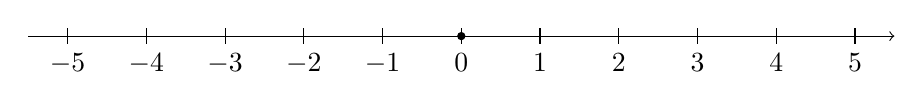
\begin{tikzpicture}[scale=1]
	\draw[->] (-5.5,0) -- (5.5,0);
	\foreach \x in {-5,-4,-3,-2,-1,0,1,2,3,4,5}
	{
		\draw (\x,0.1) -- (\x,-0.1);
		\node[below] at (\x,-0.1) {\(\x\)};
	}
	\fill (0,0) circle (1.5pt);
\end{tikzpicture}

\smallskip
\textit{Representació d'alguns nombres enters sobre la recta numèrica.}
\end{center}

Aquesta representació geomètrica permet visualitzar l'ordre dels nombres enters. Si \(a,b\in\Z\), aleshores
\[
	a<b
\]
si, i només si, el punt que representa \(a\) queda a l'esquerra del punt que representa \(b\) sobre la recta numèrica.

Per exemple,
\[
	-3<-1<0<2<5,
\]
perquè, en la recta numèrica, el punt corresponent a \(-3\) queda més a l'esquerra que el punt corresponent a \(-1\), aquest queda a l'esquerra de \(0\), i així successivament.

La distància d'un nombre enter a l'origen queda determinada pel seu valor absolut. Així, els nombres \(3\) i \(-3\) es representen en punts simètrics respecte de l'origen i es troben tots dos a distància \(3\) del punt \(0\).

\subsection{El teorema de la divisió}

Vam aprendre a fer divisions enteres fa anys per resoldre qüestions com la següent: volem repartir 15 pomes entre 7 persones de manera que cadascú rebi el màxim possible i tots la mateixa quantitat. Fent la divisió de $15$ (dividend) entre $7$ (divisor), obtenim que cadascú rep $2$ (quocient) pomes i sobra $1$ (residu). Aritmèticament, $15=7\cdot 2+1$. El resultat que vindrà ens diu que sempre podem fer això a $\Z$.

\begin{teorema}[Teorema de la divisió]\label{teo:divisio-enters}
Siguin $a,b\in\Z$, amb $b\neq 0$. Aleshores existeixen uns únics $q,r\in\Z$ tals que
\[
a=bq+r
\]
i
\[
0\leq r<|b|.
\]
El nombre $q$ s'anomena \textbf{quocient} i el nombre $r$ s'anomena \textbf{residu} de la divisió de $a$ per $b$.
\end{teorema}

\begin{prova}
Comencem amb un cas concret per il·lustrar la idea. Si $a=15$ i $b=7$, hem de trobar $q,r\in \Z$ tals que $15=7q+r$ amb $0\leq r<7$. Aïllant, $r=15-7q$, i provant valors de $q$ obtenim
\[
\ldots,29,22,15,8,1,-6,\ldots
\]
La condició $0\leq r<7$ ens dona $r=1$ i $q=2$.

Aquesta intuïció permet la prova general. Suposem primer $b>0$ i considerem el conjunt
\[
R=\{a-bq:\ q\in\Z \text{ i } a-bq\geq 0\}.
\]
Aquest conjunt és no buit. En efecte, si \(a\geq 0\), prenent \(q=0\) obtenim \(a-b\cdot0=a\geq0\), i per tant \(a\in R\). Si $a<0$, prenent $q=a$ s'obté
\[
a-b\cdot a=(1-b)\cdot a.
\]
Com que $b>0$, tenim $b\geq 1$, i per tant
\[
1-b\leq 0.
\]
Així, com que $a<0$ i $1-b\leq 0$, resulta que
\[
(1-b)\cdot a\geq 0.
\]
Per tant,
\[
a-b\cdot a\in R,
\] 
i $R\neq \emptyset$. Així doncs, $R$ és un subconjunt no buit dels enters no negatius. Identificant els enters no negatius amb nombres naturals, pel principi del bon ordre, $R$ té un element mínim. Sigui $r = \min R$. Llavors, per definició de $R$, existeix $q\in\Z$ tal que
\[
r=a-bq.
\]
Aleshores
\[
a=bq+r.
\]
A més, com que $r\in R$, tenim $r\geq 0$. Vegem ara que $r<b$. Fem-ho per reducció a l'absurd, suposem que $r\geq b$. Aleshores $r-b\geq 0$, però
\[
r-b=(a-bq)-b=a-b(q+1).
\]
Així,
\[
r-b\in R.
\]
Com que $b>0$, tenim
\[
r-b<r,
\]
cosa que contradiu que $r$ era l'element mínim de $R$. Per tant, $r<b$.
Hem provat, doncs, que si $b>0$, existeixen $q,r\in\Z$ tals que
\[
a=bq+r
\qquad\text{i}\qquad
0\leq r<b.
\]

Provem ara la unicitat en el cas $b>0$. Suposem que tenim dues descomposicions
\[
a=bq+r
\qquad\text{i}\qquad
a=bq'+r',
\]
amb
\[
0\leq r<b
\qquad\text{i}\qquad
0\leq r'<b.
\]
Volem provar que
\[
q=q'
\qquad\text{i}\qquad
r=r'.
\]

Si $q=q'$, aleshores, de
\[
bq+r=bq+r',
\]
obtenim directament
\[
r=r'.
\]

Suposem ara que $q\neq q'$. Per la tricotomia de l'ordre en $\Z$, o bé $q<q'$, o bé $q'<q$.

Si $q<q'$, aleshores existeix un enter positiu $t$ tal que
\[
q'=q+t.
\]
Substituint en la igualtat
\[
bq+r=bq'+r',
\]
obtenim
\[
bq+r=b(q+t)+r'=bq+bt+r'.
\]
Cancel\textperiodcentered{}lant $bq$, resulta
\[
r=bt+r'.
\]
Com que $b>0$ i $t>0$, tenim
\[
bt\geq b.
\]
Com que $r'\geq 0$, obtenim
\[
r=bt+r'\geq b,
\]
cosa que contradiu que
\[
r<b.
\]
Per tant, no pot ser $q<q'$.

De manera anàloga, si $q'<q$, obtindríem
\[
r'\geq b,
\]
contradient que
\[
r'<b.
\]
Per tant, tampoc no pot ser $q'<q$.

Així, necessàriament
\[
q=q',
\]
i aleshores també
\[
r=r'.
\]
Això prova la unicitat en el cas $b>0$.

Considerem ara el cas $b<0$. Aleshores
\[
-b>0.
\]
Pel cas ja demostrat, aplicat a $a$ i a $-b$, existeixen uns únics $q',r\in\Z$ tals que
\[
a=(-b)q'+r
\]
i
\[
0\leq r<-b.
\]
Com que
\[
(-b)q'=b(-q'),
\]
si definim
\[
q=-q',
\]
obtenim
\[
a=bq+r.
\]
A més, com que $b<0$, tenim
\[
|b|=-b.
\]
Per tant,
\[
0\leq r<|b|.
\]
Així queda provada l'existència també en el cas $b<0$.

Finalment, provem la unicitat en el cas $b<0$. Suposem que tenim dues descomposicions
\[
a=bq+r
\qquad\text{i}\qquad
a=bq'+r',
\]
amb
\[
0\leq r<|b|
\qquad\text{i}\qquad
0\leq r'<|b|.
\]
Com que $b<0$, tenim $|b|=-b$. Aleshores podem escriure
\[
a=(-b)(-q)+r
\qquad\text{i}\qquad
a=(-b)(-q')+r'.
\]
Com que $-b>0$, aquestes són dues descomposicions de $a$ respecte del divisor positiu $-b$, amb residus $r$ i $r'$ que compleixen
\[
0\leq r<-b
\qquad\text{i}\qquad
0\leq r'<-b.
\]
Per la unicitat ja demostrada en el cas del divisor positiu, obtenim
\[
-q=-q'
\qquad\text{i}\qquad
r=r'.
\]
Per tant,
\[
q=q'
\qquad\text{i}\qquad
r=r'.
\]

Així, per a qualsevol $a,b\in\Z$, amb $b\neq 0$, existeixen uns únics $q,r\in\Z$ tals que
\[
a=bq+r
\qquad\text{i}\qquad
0\leq r<|b|.
\]
\end{prova}

\subsection{Divisibilitat en els nombres enters}

La noció de divisibilitat també es pot estudiar en el conjunt dels nombres enters. La diferència principal respecte dels nombres naturals és que ara els divisors poden ser positius o negatius.

\begin{definicio}[Divisibilitat en $\Z$]\label{def:divisibilitat-enters}
Siguin $a,b\in\Z$, amb $a\neq 0$. Diem que $a$ \textbf{divideix} $b$, i escrivim
\[
a\mid b,
\]
si existeix $q\in\Z$ tal que
\[
b=aq.
\]
En aquest cas, diem que $a$ és un \textbf{divisor} de $b$, que $b$ és un \textbf{múltiple} de $a$, i que $q$ és el \textbf{quocient} de la divisió exacta de $b$ per $a$.
\end{definicio}

\begin{exemple}
Tenim
\[
-3\mid 12,
\]
perquè existeix $-4\in\Z$ tal que
\[
12=(-3)\cdot(-4).
\]
Per tant, $-3$ és un divisor enter de $12$.

També tenim
\[
3\mid (-12),
\]
perquè
\[
-12=3\cdot(-4).
\]
\end{exemple}

\begin{observacio}
En $\Z$, els divisors apareixen per parelles de signe. Per exemple, els divisors enters de $12$ són
\[
\pm 1,\ \pm 2,\ \pm 3,\ \pm 4,\ \pm 6,\ \pm 12.
\]
Això vol dir que
\[
1, -1, 2, -2, 3, -3, 4, -4, 6, -6, 12, -12
\]
són tots divisors de $12$ en $\Z$.
\end{observacio}

\begin{proposicio}[Propietats bàsiques de la divisibilitat en $\Z$]\label{prop:divisibilitat-enters}
Siguin $a,b,c\in\Z$, amb $a\neq 0$. Es compleixen les propietats següents:
\[
\begin{array}{ll}
\text{\textbf{(i)}} & a\mid a,\\[1mm]
\text{\textbf{(ii)}} & a\mid 0,\\[1mm]
\text{\textbf{(iii)}} & \text{si } a\mid b,\text{ aleshores } a\mid (-b) \text{ i } (-a)\mid b,\\[1mm]
\text{\textbf{(iv)}} & \text{si } a\mid b \text{ i } a\mid c,\text{ aleshores } a\mid (b+c),\\[1mm]
\text{\textbf{(v)}} & \text{si } a\mid b \text{ i } b\mid c,\text{ amb } b\neq 0,\text{ aleshores } a\mid c.
\end{array}
\]
\end{proposicio}

\begin{prova}
Demostrem cada propietat a partir de la definició de divisibilitat.

\medskip

\noindent\textbf{(i)} Com que
\[
a=a\cdot 1
\]
i $1\in\Z$, tenim
\[
a\mid a.
\]

\medskip

\noindent\textbf{(ii)} Com que
\[
0=a\cdot 0
\]
i $0\in\Z$, tenim
\[
a\mid 0.
\]

\medskip

\noindent\textbf{(iii)} Suposem que
\[
a\mid b.
\]
Aleshores existeix $q\in\Z$ tal que
\[
b=aq.
\]
Per tant,
\[
-b=-(aq)=a(-q).
\]
Com que $-q\in\Z$, obtenim
\[
a\mid (-b).
\]

D'altra banda,
\[
b=aq=(-a)(-q).
\]
Com que $-q\in\Z$, obtenim
\[
(-a)\mid b.
\]

\medskip

\noindent\textbf{(iv)} Suposem que
\[
a\mid b
\qquad\text{i}\qquad
a\mid c.
\]
Aleshores existeixen $q,r\in\Z$ tals que
\[
b=aq
\qquad\text{i}\qquad
c=ar.
\]
Per tant,
\[
b+c=aq+ar=a(q+r).
\]
Com que $q+r\in\Z$, concloem que
\[
a\mid (b+c).
\]

\medskip

\noindent\textbf{(v)} Suposem que
\[
a\mid b
\qquad\text{i}\qquad
b\mid c,
\]
amb $b\neq 0$.
Aleshores existeixen $q,r\in\Z$ tals que
\[
b=aq
\qquad\text{i}\qquad
c=br.
\]
Substituint la primera igualtat en la segona, obtenim
\[
c=(aq)r=a(qr).
\]
Com que $qr\in\Z$, concloem que
\[
a\mid c.
\]

Així queden demostrades les propietats bàsiques.
\end{prova}

\begin{observacio}
En treballar amb el màxim comú divisor dins de $\Z$, normalment es pren el representant positiu. Per exemple, tot i que $6$ i $-6$ són divisors comuns de $18$ i $24$, escrivim
\[
\operatorname{mcd}(18,24)=6,
\]
i no $-6$.
\end{observacio}
